% Recompose the supplied vector panels; the updated ratio sweep is a separate figure.
\documentclass[border=0pt]{standalone}
\usepackage{graphicx,tikz}
\begin{document}
\begin{tikzpicture}[x=1bp,y=1bp]
\path[use as bounding box] (0,0) rectangle (404,124);
\node[anchor=south west,inner sep=0] at (0,0) {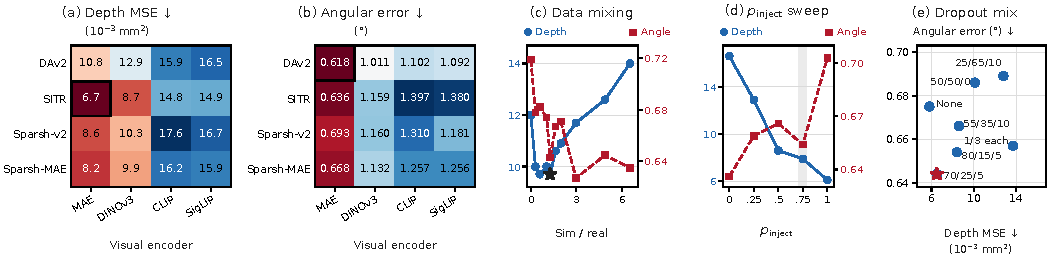
\includegraphics[width=234bp,trim=0bp 0bp 270bp 12bp,clip]{figures/figure5.pdf}};
\node[anchor=south west,inner sep=0] at (234,0) {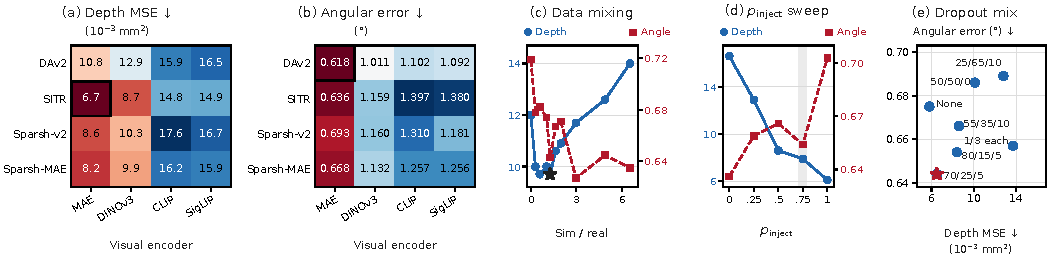
\includegraphics[width=170bp,trim=334bp 0bp 0bp 12bp,clip]{figures/figure5.pdf}};
\node[font=\sffamily\fontsize{7}{8}\selectfont] at (68,118) {(a) Depth MSE $\downarrow$};
\node[font=\sffamily\fontsize{7}{8}\selectfont] at (186,118) {(b) Angular error $\downarrow$};
\node[font=\sffamily\fontsize{7}{8}\selectfont] at (278,118) {(c) $p_{\mathrm{inject}}$ sweep};
\node[font=\sffamily\fontsize{7}{8}\selectfont] at (362,118) {(d) Dropout mix};
\end{tikzpicture}
\end{document}
